\chapter{Divine Magic}
\label{ch:divine}

This type of magic is gained through the worship of a god or goddess. Divine Magic spells come directly from the Deity and given to the character to use on their Deity’s behalf. 

The first step in learning Divine Magic is to join a religion that worships the Deity whose magic the character wants to learn.

\section{Religions}
Religions range in size from a handful of worshippers, meeting in secret to honour a dead hero of the revolution, to the millions of devotees of a world spanning sun god. There are temples where worshippers can learn Divine Magic directly from their Deity. They have rules and expectations of their worshippers and anyone found wanting is expelled from the comfort and support of the religion. 

\subsection{Religion Template}
Each religion is described using the following Religion format.
\begin{description}
\item[Name of God or Religion]
\item[Short description:] This short description briefly covers the religion’s mythology and its current place in the world.
\item[Type of Religion:] This is the type and size of religion. Great Deities are worshipped by millions and are at least acknowledged across the entire world. Major Deities are important in a specific region and have hundreds of thousands of worshipers. Minor Deities are usually the minor members of a religious pantheon appealing to a small group of specialist worshipers. Hero Religions worship dead heroes whose deeds and magic powers live on after their death.
\item[Worshippers:] The type of people who typically make up the religion membership.
\item[Worshipper Duties:] This is what the god and religion expect of its members. Break these rules and expect expulsion. On the other hand, follow these rules and promote them to others and the character will advance in the religion’s hierarchy.
\item[Religion skills:] These are skills favoured by the religion’s patron Deity and taught to its worshippers by its Priests.
\item[Religion spells:] Divine Magic that the god teaches.
\item[Special benefits:] Any bonuses to skill use or other special abilities or advantages that a worshipper gains by being a member of the religion.
\end{description}

Several examples can be seen in section~\ref{ssec:deities}.

\subsection{Worshipper Duties}
Each religion has a set of Worshipper Duties which represent the religion’s objectives in the world.

When a character does an action that fulfils one of the Worshipper Duties they gain one Improvement Point for a minor act and up to three points for a major act.

When a character does an action that goes against one of the Worshipper Duties they lose between one and three Improvement Points, depending on the grievousness of their transgression. If they have no Improvement Points left, then they start to lose Divine Magic spells learnt from the religion as a penance, on a one to one basis. The player may choose which spell to lose, but they must be ones that they have learnt from the religion.

\begin{rpg-examplebox}
Gerik the Pious acts in away that brings his god into disrepute and loses an Improvement Point. He has no Improvement Points to lose, since he has previously spent them on religion improvements, so he loses Shield 3 which he had previously learnt from the religion, which now becomes Shield 2.
\end{rpg-examplebox}

If the offending character has no Improvement Points or spells to lose, then they are excommunicated from the religion and may never join it again.

\subsection{Religion Ranks}
There are four ranks of membership: Lay members, Initiates, Priests and Holy Warriors.

\subsubsection{Lay members}
Lay members are normal worshippers of the religion. They regularly attend the temple on holy days and do their best to uphold the strictures of the religion. In return, the religion protects them as best it can, and its Priests and Initiates cast Divine Magic on their behalf. Lay members cannot learn Divine Magic. To become a lay member of a religion a character must have Lore (Religion) of at least 20\%. 

\subsubsection{Initiates}
Initiates are worshippers who have dedicated their lives to the tenents of the religion. They always attend the temple on holy days and always uphold the strictures of the religion. In return, the religion will pay ransoms if they are captured and teach the Initiate Divine Magic. Initiates can learn up to 2 Magnitude of any Divine Magic spell available to the religion. To become an Initiate a member of a religion needs a Lore (Religion) of at least 40\% and must spend two Improvement Points.

\subsubsection{Priests}
Priests are the living embodiment of their faith, instructed by their Deity to be its living representative in the mortal world. They lead the services for their temple on holy days. In return, the religion will pay ransoms if they are captured and teach them the inner secrets of their religion (this means all available Divine Magic at unlimited Magnitude). To become a Priest a character must have a Lore (Religion) and two of the cult skills at least 75\%, there must be a vacancy in the temple hierarchy, or the Priest be willing to become a missionary and establish a new temple. In addition the Player must pay five Improvement Points.

Upon becoming a Priest the character gains an Allied Spirit. This is a spirit associated with the Deity who is willing to work with one of their mortal worshipers to further the aims of the religion. The Allied Spirit is usually bound in either an animal or an item, sacred to the religion. If this item or animal is destroyed then the Allied Spirit returns to its home plane of existence. A Priest must go on a quest of repentance, which directly benefits his religion to gain a new Allied Spirit, since the Gods look dimly on Priests who lose their Allied Spirits.

An Allied Spirit starts with an INT of 2D6+6 and a POW of 3D6 and knows 3 points of Divine Magic known to the Religion. The spirit can see immaterial and invisible spirits, alerting its master to their presence in a twenty meter range. An Allied Spirit is in permanent Mind Link with its master, with a range equal to its POW x5 in meters. 

An Allied Spirit has whatever physical characteristics that its host animal or item has. Allied Spirits can be improved like player characters, by spending Improvement Points from their master’s total.


\subsubsection{Holy Warriors}
These are Holy Warriors who protect the temples and worshipers of their Deity. Not all Religions have Holy Warriors, especially those dedicated to peace, but where they do, these warriors ceaselessly crusade to protect the faithful and punish the Religion’s enemies. Like Priests they are expected to uphold the Worshipper duties unfailingly. Also, as the religion’s warriors, they are expected to take up arms against any aggressor who attacks its worshippers or the religion’s Temples.

These warriors are incredibly useful to the cult they belong to, which will always pay any ransom or make a rescue attempt when a Holy Warrior is captured. In addition they teach them any Divine Magic known to the religion.

The minimum requirement to become a Holy Warrior is to have Lore (Religion) of at least 50\% and a Weapon Skill of 75\% in the Religion’s holy weapon, usually the weapon that is most associated with the Deity that the Religion worships. In addition the Player must pay five Improvement Points.

When someone becomes a Holy Warrior they are gifted a specially consecrated weapon, that gives them a bonus when fighting to defend fellow worshippers, religion temples, and when attacking enemies of their faith.  This bonus is usually +20\% to the appropriate weapon skill and double damage when fighting for their Religion. All damage done by such weapons is considered magical.

They also gain armour, which is magically blessed by the Religion’s Deity. Normally, this is at least double the normal AP of the armour type used, and it may have additional powers depending on the Deity.


\subsection{Player Character Priests}
Priests and Holy Warriors don’t just hang around their Temples doing their duties. They have plenty of Initiates and lay worshippers to do the more mundane administrative tasks, such as collecting tithes and feeding the poor. As player characters, their lives are more interesting and the source of constant adventuring on behalf of their religion. Some of the quests that they might get involved in are as follows:
\begin{rpg-list}
\item Going out and converting the unbelievers (or those who believe in the wrong Deity).
\item Actively fighting the enemies of the religion.
\item Recovering long-lost symbols and powerful artefacts of the faith. 
\item Attending a cross-faith to deal with all the politics and misunderstanding to come to a consensus about what to do about a common enemy.
\item Rushing to the aid of an embattled and besieged town of his faithful believers beset by enemies or some other form of spiritual peril.
\item Visiting the hinterlands to provide spiritual guidance and duties to those in need
\item Traveling to a distant Holy Mountain to commune directly with their Deity or otherwise performing idealistic inspirational acts, or to prove their worth.
\item Going on special mission, where success depends on Divine Magic.
\item Traveling as a special envoy of the Religion to show due deference to the King / Priest / High Emperor.
\end{rpg-list}


\subsection{Deity Examples}
\label{ssec:deities}
The following Religions are intended as examples or templates for your own creations or as simple pick up and play religions, that can be elaborated and detailed as a campaign progresses.

\subsubsection{The Night Mistress}
When the Sun Lord sleeps, the mistress of the Night stealthily creeps up from the Underworld to play.  Whether her games are harmful or beneficial depends on the person's view of the dark.

\begin{description}
\item[Type of Religion:] Great
\item[Worshippers:] Monsters of the Underdark, Thieves, Outcasts from society.
\item[Worshipper Duties:] Banish the light! Preserve the sanctity of Dark regions, prevent the forces of light invading the underworld. Remain mysterious and unfathomable.
\item[Religion skills:] Deception, Ranged Combat, Unarmed Combat
%\item[Magic:] Darkwall, Enhance Deception, Extinguish.
\item[Divine Magic:] All common spells, Call Shade, Fear.
\item[Special benefits:] +20\% to Deception during the Night.
\end{description}


\subsubsection{The Sun King}
The bright blazing ruler of the day. The everlasting source of life and light. To some cultures he is the Imperial Emperor, whose sacred word is to be obeyed without question. Also a source of healing and resurrection.

\begin{description}
\item[Type of Religion:] Great
\item[Worshippers:] Emperors, Charismatic Leaders
\item[Worshipper Duties:] Banish the dark, Guide the masses.
\item[Religion skills:] Healing, Close Combat, Ranged Combat, Influence.
%\item[Magic:] Enhance Influence, Fire Missile?, Fire Weapon?, Heal, Light, Multi Missile.
\item[Divine Magic:] All common spells, Call Salamander, Divine Heal, Resurrect, Sun Spear, Sun Disc, Radiant Appearance.
\item[Special benefits:] +20\% to Influence skills when dealing with lower social classes.
\end{description}



\subsubsection{The Sky Lord}
Arrogant and aloof, the Sky Lord brings storm and rain at the behest of his elder ruling brother the Sun King.  He strains at the unreasonable laws that bind him to his brother’s authority and is a constant rebel. In some lands he has cast off his brother’s chains and is acknowledged as the King of the Gods.

\begin{description}
\item[Type of Religion:] Great
\item[Worshippers:] Barbarians
\item[Worshipper Duties:] Ride the storm!, Fight against Tyrants, Stay free.
\item[Religion skills:] Close Combat, Natural Lore.
%\item[Magic:] Fanaticism, Extinguish, Vigour, Weapon Enhance.
\item[Divine Magic:] All common spells, Berserk, Call Sylph, Lightning Strike, Whirlwind, Enhance Machismo.
\item[Special benefits:] Suffers no penalty when doing skill tests in rainy or windy conditions.
\end{description}



\subsubsection{The Earth Mother}
The all embracing and loving Earth Mother is known throughout the world. Some people believe that she is the world itself. She is the source of all nature’s bounty, which clothes and feeds mankind, but also has a savage side that expresses itself in hurricanes, tidal waves and other natural disasters. 

\begin{description}
\item[Type of Religion:] Great
\item[Worshippers:] The religion is made up of people and creatures who live off the land. In civilised areas these are the peasants who farm the land and the woodsmen who hunt and gather in the forests. In the wilderness the Elves, Satyrs and Fey worship her. She is found wherever creatures have an acknowledged connection with nature.
\item[Worshipper Duties:] Respect the Earth. Don’t foul or pollute the environment. Practice the peaceful cut, a small prayer said in thanks to the animal spirit before killing it for food. The prayer ensures its return to the Earth Mother and through the cycle of rebirth into the world. 
\item[Religion skills:] Healing, Nature Lore, Resilience.
%\item[Magic:] Heal, Protection
\item[Divine Magic:] All common spells, Absorption, Berserk, Heal Body.
\item[Special benefits:] Any member of this cult gains a +20\% bonus to their Nature Lore, due to their connection to Nature, which they gain through their relationship with the Earth Mother.
\end{description}


\subsubsection{The Death Goddess}
Banished to the Underworld by the Sun King for a heinous crime, the Sun King’s sister is a twisted force that rails against the authority of her brother. Unable to leave the Underworld, she and her agents take that which is most precious to her brother, the very souls of his subjects, the living. She does this upon their physical death. Those judged unworthy by the Sun King, denied bliss in Eternal Golden Heaven, are taken by her cold embrace, into the Underworld. 

\begin{description}
\item[Type of Religion:] Great
\item[Worshippers:] The morbidly insane, Mercenaries, Graveyard attendants, Assassins.
\item[Worshipper Duties:] Respect the dead, Put down the Undead.
\item[Religion skills:] Close Combat, Undead Lore. 
%\item[Magic:] Demoralise, Spirit shield, Weapon Enhance.
\item[Divine Magic:] All common spells, Call (Undead), Death March, Resurrect, Touch of Death.
\item[Special benefits:] +20\% when inspecting corpse to determine time and cause of death.
\end{description}


\subsubsection{The Lord of Knowledge}
He is the Great Sage of Heaven, who exists only to drink in all the facts and information about the world. His book-loving followers emulate him, making a living by running Knowledge markets and selling advice and information.

\begin{description}
\item[Type of Religion:] Major
\item[Worshippers:] Explorers, Librarians, Scholars, Detectives.
\item[Worshipper Duties:] Find out new knowledge, catalogue and record information, maintain public libraries, punish knowledge thieves, remain unbiased and impartial.
\item[Religion skills:] Lores of various types, Influence, Languages.
%\item[Magic:] Detect X, Mindspeech.
\item[Divine Magic:] All common spells, Find X of various types, Soul Sight, See Past.
\item[Special benefits:] +20\% when using a Library to find information.
\end{description}



\subsubsection{The Trickster}
Culture hero or culture villain? This Deity aims to amuse him/herself by playing pranks on those who, in its opinion, deserve to be shamed before their peers. In some cultures the Trickster is revered as a Sacred Clown, who mocks authority when it is high-and-mighty and not working in the interest of the people. In others, he is outlaw, defying the Divine Right of the rulers to oppress the people.

\begin{description}
\item[Type of Religion:] Major
\item[Worshippers:] Thieves, Village idiots, non-conformists.
\item[Worshipper Duties:] Play pranks on the pompous and foolish.
\item[Religion skills:] Deception, Ranged Combat.
%\item[Magic:] Befuddle, Hinder.
\item[Divine Magic:] All common spells, Illusion, Reflection, Purity, Wax Effigy, Puppet, Jigsaw.
\item[Special benefits:] +20\% Deception when playing pranks.
\end{description}



\subsubsection{The Merchant}
He is a constant traveller, who gains joy by communicating with the new friends that he meets along the way. Long ago he learnt the art of commerce, as a way of making his contacts happy and a way of learning about the workings of the cultures he encounters. His followers know that a mule, a bag of shiny things, and a warm accepting smile, is all that is needed to open up a world of opportunity and reward.

\begin{description}
\item[Type of Religion:] Major
\item[Worshippers:] Merchants, Heralds, Traders, Shopkeepers.
\item[Worshipper Duties:] Spread the word to new places, Enrich both yourself and your temple. 
\item[Religion skills:] Influence, Perception, Ride, Drive, Languages.
%\item[Magic:] Clear the Path, Enhance Influence, Enhance Perception.
\item[Divine Magic:] All common spells, Treasury, Ward Camp, Create Crystal Ship.
\item[Special benefits:] +20\% when using Perception or Influence as part of a financial deal.
\end{description}


\subsubsection{The Hearth Goddess}
This down to earth Deity is a daughter of the Earth Goddess who chose to live in the urban centres of mortals. She looks after the home. Her name is invoked to maintain domestic harmony and fertility.

\begin{description}
\item[Type of Religion:] Minor
\item[Worshippers:] House keepers and owners.
\item[Worshipper Duties:] Keep a clean and orderly home.
\item[Religion skills:] Craft, Influence.
%\item[Magic:] Heal, Enhance Craft.
\item[Divine Magic:] All common spells, Block Fertility, Enhance Fertility, Repair and Replace.
\item[Special benefits:] +20\% to any skill test in the character’s home.
\end{description}


\subsubsection{The Lord of War}
He is a blood-soaked Deity of violence and conflict. He is mentor and master to both the high-and-mighty General and the rank-and-file soldier. In civilized cultures he is worshipped through arcane ritual, where armies receive his blessing before battle. Amongst the Barbarians he is invoked through deed, in the fire of the battle itself.

\begin{description}
\item[Type of Religion:] Great
\item[Worshippers:] Generals, soldiers.
\item[Worshipper Duties:] Fight hard, Fight to win, Fight!
\item[Religion skills:] Close Combat, Dodge, Ranged Combat, Unarmed Combat.
%\item[Magic:] Coordination, Fanaticism, Strength, Vigour, Weapon Enhancement. 
\item[Divine Magic:] All common spells, Shield, Rout, True (Weapon), Unstoppable Charge, Ward Camp.
\item[Special benefits:] +20\% for any test when leading others into Combat.
\end{description}


\subsubsection{The Healer Goddess}
The White One will heal anyone, regardless of behaviour and allegiance. Her white-robed worshippers are found not only in settlements but also in the wagon-trains of armies. Healing gives even the most violent individual the chance to turn their life around and become a Warrior for Peace.

\begin{description}
\item[Type of Religion:] Major
\item[Worshippers:] Healers, Doctors
\item[Worshipper Duties:] Heal anyone regardless of outlook on life, maintain areas of sanctuary.
\item[Religion skills:] Healing, Perception, Influence.
%\item[Magic:] Heal
\item[Divine Magic:] All common spells, Divine Heal, Resurrect.
\item[Special benefits:] +20\% to all Healing attempts.
\end{description}


\subsubsection{The Sea Goddess}
She is the avaricious sister of the Earth Goddess, who is either the elder or younger sibling depending who you talk to. She constantly wars with her sister for surface area on the planet. In some places her tides eat the land and swallow remote islands. In others her waters relent and give back dry land previously sunk in Ancient times. Any sailor is wise to ask her permission before travelling across her watery realm.

\begin{description}
\item[Type of Religion:] Great
\item[Worshippers:] Sailors, fishermen, mermen, creatures of the sea.
\item[Worshipper Duties:] Respect the sea, ensure the goddess’ permission is sought by sailors. 
\item[Religion skills:] Sailing, Natural Lore
%\item[Magic:] Detect Treasures of the Sea, Water Breath.
\item[Divine Magic:] All common spells, Call Undine, Breathe Water.
\item[Special benefits:] +20\% to all sailing checks made at sea, and Athletics checks made to swim. 
\end{description}


\subsubsection{Chaos}
The writhing thing that is Chaos, strains and buckles on the boundaries of creation. Outside of the ordered universe, it howls to get in, and when it breaks through the cracks in reality it causes change and the warping of nature. 

\begin{description}
\item[Type of Religion:] Great
\item[Worshippers:] The insane, its foul monstrous spawn.
\item[Worshipper Duties:] Erode the very fabric of reality, destroy beauty, inflict pain on the living.
\item[Religion skills:] None.
%\item[Magic:] Befuddle, Countermagic, Demoralise, Disruption, Ignite.
\item[Divine Magic:] All common spells, Fear, Madness.
\item[Special benefits:] Immune to any kind of Mind Control magic.
\end{description}


\subsubsection{The Moon Hag}
There is an old woman who lives on the moon. She is the queen of the witches and all the spirits who live on the dark side of the moon. She is an enigma who will send you mad if you offend her sensibilities. 

\begin{description}
\item[Type of Religion:] Minor
\item[Worshippers:] Magicians, Astronomers.
\item[Worshipper Duties:] Observe the moon, maintain the mystery of the moon amongst non-religion members, study moon mysteries.
\item[Religion skills:] Natural Lore.
%\item[Magic:] Call (Magic, Spell spirit ), Counter magic.
\item[Divine Magic:] All common spells, Reflection, Mindblast, Mindlink, Madness.
\item[Special benefits:] +20\% to any skill roll when dealing with Moon spirits.
\end{description}


\subsubsection{The Huntress}
The Divine Huntress stalks the land. In primitive and barbaric societies she is the patron of those who go into the wilderness to bring back essential meats to the tribe. In more civilised areas, she takes on the character of the supreme risk-taker, looking for more and more fabulous and exotic prey for glory and renown.

\begin{description}
\item[Type of Religion:] Minor
\item[Worshippers:] Hunters, Big Game Hunters.
\item[Worshipper Duties:] Be true to the hunt, do not deplete the hunting grounds, capture poachers.
\item[Religion skills:] Deception, Ranged Combat, Nature Lore.
%\item[Magic:] Multi Missile, Coordination, Clear Path, Speedart.
\item[Divine Magic:] All common spells, Sureshot, True (Bow or Spear).
\item[Special benefits:] +20\% Deception when stalking prey.
\end{description}



\subsection{Learning Divine Magic}
Divine Magic can be taught only to members of a religion with an appropriate Lore (Religion) skill and be of Initiate, Priest or Holy Warrior status (each rank requiring Improvement Points).


\subsection{Learning Spells}
A character with access to the Divine Magic discipline can learn new spells by paying a cost in Improvement Points, equal to twice the Magnitude of the spell, to the Deity. This may be done in an incremental fashion, i.e. the player buys Shield 1 for two Improvement Points and then later increases this to Shield 3, by spending an additional four points. These points are not regained, even when the character leaves the religion.


\subsection{Casting Spells}
A character must be able to gesture with his hands and be able to chant in order to cast a spell. Whenever a spell is cast using Divine Magic, there will always be a sight and sound that nearby creatures can detect, be it a flash of light, a crack of thunder or a shimmering in the air. The exact effects, are up to the Gamemaster and Player to decide but will automatically be detected by any creatures within ten times the Magnitude of the spell, in metres. 

Casting Divine Magic is automatically successful. No dice need be rolled, no chances of a fumble or critical either.

\subsubsection{Power Points}
Divine Magic does not cost any Power Points when it is cast.

\subsubsection{Casting Time}
Divine Magic spells always take only a single combat Action to cast and takes place on the Combat Order of the character casting the spell.

Distractions or attacks on the spellcaster as he casts will either automatically ruin the spell (if the spellcaster is blinded or disarmed, or suffers a Major Wound) or require Persistence tests for them to maintain concentration on the spell. 

\subsubsection{Regaining Cast Divine Magic}
Each Divine Magic spell may be cast only once, after which the character must return to a temple and pray or take part in a worshiping ceremony on the religion’s holy day to regain use of the spell. Thus, normally, Divine Magic is regained during the downtime between adventures.

In-game characters may regain Divine Magic by one of two ways.
\begin{rpg-list}
\item Each time the character successfully performs a worshipper duty, the character regains the choice of one of their spent spells.
\item They may also call on their deity and spend a Hero Point to regain a spent spell of their choosing.
\end{rpg-list}


\subsubsection{Limitations}
Divine Magic spells do not stack, i.e. Shield 1 plus Shield 2 does not give the protection of a Shield 3 spell.

\subsubsection{Dismissing Spells}
A caster can dismiss any Permanent or Duration Divine Magic spell(s) he has cast as a single combat action. Ceasing to cast a Concentration spell is immediate and not a Combat Action.


\subsubsection{Splitting Magnitude}
Divine Magic allows the caster to ‘split’ a spell’s Magnitude into multiple spells. For instance, if the caster knows the Absorption spell at Magnitude 3, he may choose to cast it as a single Magnitude 3 spell, or he may split it into three Magnitude 1 Absorption spells, or one Magnitude 1 and one Magnitude 2 Absorption spell. The split spells are treated as separate instances and are cast separately.

\subsubsection{The Power of Divine Magic}
When in a direct contest with other forms of magic, Divine Magic is considered to have double its normal Magnitude.

\subsubsection{Common Divine Magic}
The following spells are listed as ‘All’, since all Cults teach them:

Consecrate, Create Blessed Item, Create Idol, Dismiss Magic, Divination, Excommunicate, Exorcism, Extension, Find X, Mindlink, Soul Sight, Spirit Block, Spiritual Journey.

\subsection{Divine Intervention}
Characters also gain the ability to call for Divine Intervention. 
A character who is an Initiate, or higher, can call upon his Deity for Divine Intervention whenever he faces a desperate situation. He may even do so if dead or unconscious, as long as it is called for in the instant that consciousness fades or death occurs. When Divine Intervention is requested, roll 1D100. If this roll is equal to or less than the character’s POW, the call for aid is answered. However, the gods demand a heavy price for their help and the character will suffer a permanent loss of POW equal to the 1D100 roll, if they are successful. If the character’s POW is reduced to 0 by this, their soul is taken to serve the god directly, effectively killing the character permanently (though their request will still be granted). 

A character can only call for Divine Intervention once per month, whether he is successful or not. 

Divine Intervention can take many forms and the following can be considered guidelines: 
\begin{rpg-list}
	\item Allow the character to cast any religion spell (of that Deity) at any Magnitude.
	\item Allow a religion spell to affect every worshipper of the god within the character’s line of sight. 
	\item Bring back to life a worshipper (who may not be the character calling for Divine Intervention). 
\end{rpg-list}

Various ‘divine’ effects are also possible depending on the nature of the character’s Deity. Examples could include creating a fog to allow the character to escape from enemies, doubling their STR to defeat a powerful enemy or causing a river to break its banks to stall an invading army. 

Divine Intervention cannot be used to directly harm or slay mortal creatures. Gods will refuse to aid non-worshippers and their effects will be related to their sphere of influence. 


%\subsection{Regaining Divine Magic Spells}
%Divine Magic spells represent the channeling of Divine Power into the mortal world. The caster is the vessel and initiator only and thus does not spend any Power Points to cast them. At higher Magnitudes Divine spells are very powerful and thus the mechanics of regaining them is more difficult than other casters. Divine Magic users have to regain their magic from their Deity, with whom they must be on good terms. 

%For each hour of rest, meditation or ceremonial communion with the character’s Deity, 1 Point of Divine magic is regained and the caster must choose exactly which spells he regains at the end and at what Magnitude, up to 2 Magnitude. Of course no spell can be chosen more than once. To regain Magnitude 3 and higher the caster needs to either pray in a temple or participate in a worshipping ceremony on one of the Holy Days of the Deity. That means that the character must be prepared to be without high magnitude Divine spells for long periods of time.

%Of course, at the Gamemaster's discretion, spells can be regained at other important occasions. For example, performing an important deed that is aligned with a Deity's creed could allow the character to instantly regain high Magnitude spells.



\subsection{Spell Traits}
The traits used by Divine Magic spells are detailed below. 

\begin{description}
	\item[Area (X):] The spell affects all targets within a radius specified in metres.
	\item[Concentration:] The spell’s effects will remain in place so long as the character concentrates on it. Concentrating on a spell is functionally identical to casting the spell, requiring the caster to continue to gesture with both arms, chant, and ignore distractions.
	\item[Duration (X):] The spell’s effects will stay in place for the number of minutes indicated. 
	\item[Instant:] The spell’s effects take place instantly. The spell itself then disappears. 
	\item[Magnitude (X):] The strength and power of the spell.
	\item[Permanent:] The spell’s effects remain in place until they are dispelled or dismissed.
	\item[Progressive:] This indicates that the spell can be learnt and cast at greater levels of Magnitude than the minimum.
	\item[Ranged:] Ranged spells may be cast upon targets up to a maximum distance of the character’s POW x 5 in metres.
	\item[Resist (Dodge/Persistence/Resilience):] The spell’s effects do not take effect automatically. The target may make a Dodge, Persistence or Resilience test (as specified by the spell) in order to avoid the effect of the spell entirely. Note that Resist (Dodge) spells require the target to be able to use Reactions in order to Dodge. In the case of Area spells, the Resist (Dodge) trait requires the target to dive in order to mitigate the spell’s effect. 
	\item[Touch:] Touch spells require the character to actually touch his target for the spell to take effect. The caster must remain in physical contact with the target for the entire casting.
	\item[Religion:] The type of religion that offers this spell to it’s worshippers. If the religion is listed as All, the spell is a Common spell available in all religions. The religion’s description will help determine which spells should or should not be available. 
\end{description}

\section{Spells}

%\begin{samepage}
\begin{rpg-spell}
{Absorption}
{Duration 15, Magnitude 1, Progressive, Touch\\{[Religions: Earth, Night]}}

This spell absorbs incoming spells aimed at the target or his equipment, converting their magical energy into Power Points which are then available to the target. Once cast on a subject, Absorption will attempt to absorb the effects of any spells cast at the target. It will not have any effect on spells that are already affecting a character. The effects of Absorption depend on the relative Magnitude of both itself and the incoming spell. If the Absorption's Magnitude is equal or greater to the incoming spell then it is absorbed and Absorption remains; if not Absorption is eliminated and the incoming spell takes effect. Any spell absorbed by this spell is cancelled and has no effect. 

A character may not accumulate more Power Points than his POW while Absorption is in effect – excess Power Points garnered through Absorption simply vanish. Absorption is incompatible with Reflection, Shield and Spirit Block.
\end{rpg-spell}
%\end{samepage}

%\begin{samepage}
\begin{rpg-spell}
{Berserk}
{Duration 15, Magnitude 2, Touch\\{[Religions: Beasts, War]}}

The recipient of this spell is overcome with bloodlust, causing them to disregard their own safety and loyalties but imbuing them with tremendous stamina and combat ability. 

The recipient will automatically succeed any Resilience test for the duration of the spell. The recipient also automatically succeeds at any Fatigue tests and cannot be rendered unconscious. The Close Combat skills of the recipient receive a +40\% bonus for the spell’s duration. 

However, the subject may not Parry, Dodge or cast any magic spells while under the influence of Berserk. Normally, the recipient remains in the Berserk state for the entire 15 minute duration of the spell, but Gamemasters may allow a Berserk character to shake off the effects with a Persistence test modified by -40\%. At the end of the spell, the recipient immediately becomes Fatigued. 

Berserk may not be combined with Fanaticism and in such cases Berserk will always take precedence. 
\end{rpg-spell}
%\end{samepage}

%\begin{samepage}
\begin{rpg-spell}
{Block Fertility}
{Magnitude 3, Permanent\\{[Religions: Earth]}}

While this spell is in place, the recipient is unable to conceive. This can be seen as a blessing or a curse depending on the view of the recipient. The spell can be dispelled by the caster whenever they want. Otherwise the effect of the spell is permanent. 
\end{rpg-spell}
%\end{samepage}

%\begin{samepage}
\begin{rpg-spell}
{Breath Water}
{Duration 15, Magnitude 2, Touch\\{[Religions: Sea, Water]}}

This spell allows an air-breathing creature to breathe water for the spell’s duration (the subject will still be able to breathe air as well). It may also be used upon a water-breathing creature to allow it to breathe air. 
\end{rpg-spell}
%\end{samepage}

%\begin{samepage}
\begin{rpg-spell}
{Call (Elemental)}
{Magnitude 1, Permanent, Progressive\\{[Religions: Any with affinity to elements]}}

This spell summons and binds to the service of the caster an elemental from another plane of existence, of a size dependant on the Magnitude of the spell:
1=Small, 2=Medium, 3=Large, 4=Huge (for more details on Elementals see page~\pageref{monster:elemental}). The elemental stays under the control of the Priest until it is killed or the Call spell is dispelled. 
	
To be successfully cast the spell requires an equal volume of the same material that the elemental is made up of. For example, a Large Undine (Water elemental) requires a pool of water of at least 50 m3 before it can be summoned.
\end{rpg-spell}
%\end{samepage}

%\begin{samepage}
\begin{rpg-spell}
{Call (Undead)}
{Magnitude 1, Permanent, Progressive\\{[Religions: Evil, Death]}}

This spell reanimates a dead human corpse and turns it into an undead creature, of a type determined by the Magnitude of the spell:
1=Skeleton, 2=Zombie, 5=Ghoul, 8=Vampire. The undead creature stays under the control of the Priest until it is killed or the Call spell is dispelled.
\end{rpg-spell}
%\end{samepage}

%\begin{samepage}
\begin{rpg-spell}
{Consecrate}
{Area Special, Magnitude 1, Permanent, Progressive\\{[Religions: All]}}

This spell is as much a part of a temple’s foundation as is its cornerstone, but may actually be cast almost anywhere. It creates a sphere with a radius of ten metres per point of Magnitude. The consecrated sphere is sacred to the caster’s god. Consecrate by itself does nothing to keep outsiders at bay, but the caster of the spell will know immediately if a spell, spirit or someone who is not a lay member of his cult crosses the boundaries of the Consecrate spell.
\end{rpg-spell}
%\end{samepage}

%\begin{samepage}
\begin{rpg-spell}
{Create Blessed Items}
{Area Special, Magnitude 1, Permanent, Progressive\\{[Religions: All]}}

This spell allows the caster to create items which store Divine Magic spell(s) that are blessed by a Priest with power from the Deity. Only Priests and High Priests can create blessed items. The enchanter forgets the spell(s) he blesses the item with (i.e. he has to relearn it with Improvement Points).

The wielder of the item can cast the spell(s) the item is blessed with, but once the item’s power is discharged then it must be reconsecrated at a temple of the religion. The consecration takes as many hours as the Magnitude of the spell. If the Magnitude of the spell is higher than two, the consecrating team must have at least one Priest. The wielder must be a member of either the religion that created the blessed item or an allied religion. 

Blessed items become protected by the religion’s Deity and can not be broken by normal non-magical means. 
\end{rpg-spell}
%\end{samepage}

%\begin{samepage}
\begin{rpg-spell}
{Create Idol}
{Magnitude 4\\{[Religions: All]}}

This spell requires an image of the caster’s god worth 100 GPs to be made, while a Priest reads from the sacred texts of the Deity telling the tales and myths. This stores the god’s spells, and can be used by Priests and Initiates to regain spells and can be used by Lay Members to receive lessons, via visions, upon touching the idol. Such visions will increase the Religion skill of a Lay Member by 1D10\% when they are repeatedly exposed to them. 
\end{rpg-spell}
%\end{samepage}

%\begin{samepage}
\begin{rpg-spell}
{Create Crystal Ship}
{Magnitude 4, Duration the length of the voyage\\{[Religions: Merchant]}}

	From out of the air coalesces a Crystal Ship, a magical vessel that sails through the air to a single destination preordained by the caster. The caster need never have been there, but the casters’ Deity must know of it. The ship is about the size of a merchant cog (one-masted as described in table~\ref{tab:ship-types}, page~\pageref{tab:ship-types}) and is fitted with no weapons. Although the ship heads steadily towards the destination, at a rate of 100 km a day, the fine maneuvering of the ship is managed by the mental thoughts of the caster.
\end{rpg-spell}
%\end{samepage}

%\begin{samepage}
\begin{rpg-spell}
{Death March}
{Magnitude 4, Duration 1 Day\\{[Religions: Death]}}

This spell raises the local spirits of a settlement and makes them parade up and down the main road of that settlement, for a twenty four hour period. Most of the dead will be in the form of ghosts, but the freshly dead will rise as Zombies, and those who still have bones in the cemetery will rise as Skeletons. Both types of physical dead will attack any living beings that get in their way. 
\end{rpg-spell}
%\end{samepage}

%\begin{samepage}
\begin{rpg-spell}
{Dismiss Magic}
{Instant, Magnitude 1, Progressive, Ranged\\{[Religions: All]}}

Dismiss Magic may be cast against either a general target or a specific spell. Dismiss Magic will eliminate a combined Magnitude of spells equal to its own Magnitude, starting with the most powerful affecting the target. If it fails to eliminate any spell (because the spell’s Magnitude is too high), then its effects immediately end and no more spells will be eliminated. A spell cannot be partially eliminated, so a target under the effects of a spell whose Magnitude is higher than that of Dismiss Magic will not have any spells currently affecting it eliminated. Remember that Divine Magic's Magnitude counts as double vs non-divine magic.
	
The caster can also target Dismiss Magic against a single specific spell. 
Dismiss Magic may be fired as a Reaction, but only when another spell is cast within Dismiss Magic’s Range that the character wishes to counter. A successful Dismiss Magic disrupts the other spell and nullifies it. 
\end{rpg-spell}
%\end{samepage}

%\begin{samepage}
\begin{rpg-spell}
{Divination}
{Instant, Magnitude 1, Progressive\\{[Religions: All]}}

For each point of Magnitude of this spell the caster can ask one question of their Deity, which they must answer to the best of their ability. A Deity can only answer questions it knows about and that falls within its sphere of power. For example, a Mountain God will know exactly what is going on its slopes at any given time, but will be completely ignorant about the Ocean.

Gods will also commonly ask for a sacrifice of an animal or precious object worth one Gold Piece per question asked. Particularly cruel and bloodthirsty deities will demand blood sacrifices of sentient beings.
\end{rpg-spell}
%\end{samepage}

%\begin{samepage}
\begin{rpg-spell}
{Divine Heal}
{Instant, Magnitude 1, Progressive, Touch\\{[Religions: Earth, Fertility]}}

This powerful spell instantly heals a number of Hit Points equal to its Magnitude times four. It also cures any natural deseases and poisons. Each casting of Divine Heal will heal one Major Wound and if necessary will reattach or regenerate damaged limbs and organs.  
\end{rpg-spell}
%\end{samepage}

%\begin{samepage}
\begin{rpg-spell}
{Enhance Fertility}
{Magnitude 3, Permanent\\{[Religions: Earth, Fertility]}}

This spell makes any one creature more fertile than normal. If it is an animal that has multiple offspring then it doubles the number. For creatures who have singular births, it guarantees conception and birth of the offspring. This spell negates the effects of any Block Fertility spell. 
\end{rpg-spell}
%\end{samepage}

%\begin{samepage}
\begin{rpg-spell}
{Enhance Unit}
{Magnitude 3, Duration 6 Hours\\{[Religions: War]}}

For the duration of this spell a troop of up to thirty soldiers gain +1D6 damage. Also they cannot be routed or affected by any mind control magic (such as Befuddle).
\end{rpg-spell}
%\end{samepage}

%\begin{samepage}
\begin{rpg-spell}
{Excommunicate}
{Magnitude 5, Permanent, Resist (Persistence)\\{[Religions: All]}}

This spell severs the mystical link an Initiate enjoys with their god, causing the target of the spell to immediately and permanently lose all Divine Magic from the caster’s religion. The target will never again be able to learn or use Divine Magic spells from the religion, though they will still be able to use Lore (Religion) for purely academic purposes. 

This spell must be cast by a Priest and takes one hour to cast. The Initiate need not be present. The spell can only be cast on Initiates or higher and who worship the same god of the caster of the spell.
\end{rpg-spell}
%\end{samepage}

%\begin{samepage}
\begin{rpg-spell}
{Exorcism}
{Concentration, Magnitude 3\\{[Religions: All]}}

A Divine Magic caster can draw out a spirit currently possessing a mortal being by using this spell. Whether the possession is dominant or covert is immaterial.

This spell forces a possessing spirit into Spirit Combat. The caster uses his Religion (Own) as the attacking skill in the opposed contest, as this represents the strength of their faith. If the caster is successful in defeating the spirit, it is cast out of the victim and flees. If the caster fails, the spirit remains in the possessed victim.
\end{rpg-spell}
%\end{samepage}

%\begin{samepage}
\begin{rpg-spell}
{Extension}
{Duration Special, Magnitude 1, Progressive\\{[Religions: All]}}

This spell lengthens the duration of any Divine Magic spell with the Duration trait. Extension, and the spell it is extending, are cast simultaneously by the caster – this is an exception to the normal rule that only one Divine Magic spell may be cast during a single Combat Round. 

Each point of Magnitude of the Extension spell doubles the target spell’s duration. Thus, a Magnitude 1 Extension increases Breathe Water’s Duration to 30 minutes, a Magnitude 2 increases it to one hour, Magnitude 3 increases it to two hours, Magnitude 4 increases it to four hours, and so on.
\end{rpg-spell}
%\end{samepage}

%\begin{samepage}
\begin{rpg-spell}
{Fear}
{Instant, Magnitude 1, Ranged, Resit (Persistence)\\{[Religions: Chaos, Night]}}

This spell causes the target to be gripped with overwhelming fear. Fear has no effect on unconscious targets, targets without an INT Characteristic or targets that are currently under the influence of a Fear spell. The effect depends on the result of the Persistence check as follows:
\begin{description}
\item[Fumble:] Victim instantly loses half original Hit Point damage (enough to cause a Major Wound) as its heart falters. 
\item[Failure:] Victim flees in screaming terror for a number of Combat Rounds equal to 20 minus its POW (minimum of one Combat Round). Victim will not engage in combat unless forced to and will use the Run Combat Action whenever possible (unless a faster mode of egress is available). 
\item[Success:] Victim is shaken and disturbed, suffering a –20\% penalty to all skill tests for a number of Combat Rounds equal to 20 minus its POW (minimum of one Combat Round).
\item[Critical:] Victim is unaffected by the spell and cannot be affected by further Fear spells for a number of Combat Rounds equal to its POW.
\end{description}
\end{rpg-spell}
%\end{samepage}

%\begin{samepage}
\begin{rpg-spell}
{Find X}
{Duration 15, Magnitude 1, Ranged\\{[Religions: All]}}

This is actually several spells, though they all operate in a similar fashion, which allow the caster to locate the closest target of the spell within its range. This effect is stopped by a thick substance such as metal, earth or stone if it is at least one metre thick. It is also blocked by Absorption, though the caster will know the target is somewhere within range (though not its precise location) and that it is being protected by Absorption. Unlike the Magic Detect spells, the Find spells do not require concentration on the part of the caster – they simply function and alert them to the presence of whatever they are meant to locate. The separate Find spells are listed below. 
\begin{description}
\item[Find Enemy:] Gives the location of one creature who intends to harm the caster. 
\item[Find Magic:] Gives the location of the nearest magic item, magical creature, or active spell. 
\item[Find (Species):] Each Find Species spell will give the location of the nearest creature of the specified species. Examples of this spell include Find Goblin, Find Dwarf and Find Horse
\item[Find Substance:] Each Find Substance spell will give the location of the nearest substance of the specified type. Examples of this spell include Find Coal, Find Gold and Find Wood. 
\end{description}
The Gamemaster should provide the rough power of the detected subject (‘weak magic’ or ‘rich gold lode’). 
\end{rpg-spell}
%\end{samepage}

%\begin{samepage}
\begin{rpg-spell}
{Illusion}
{Duration 15, Magnitude 1, Progressive, Ranged\\{[Religions: Moon, Trickster]}}

This spell creates an illusion based on all five senses. The illusion will seem real and solid unless the person looking at it succeeds in a Perception test. If the viewer succeeds in a Perception test and the Illusion could usually cause damage if believed in, it can no longer cause damage to that character. As soon as a viewer disbelieves the illusion it becomes insubstantial and ghost-like to him.

The Size and the strength of the illusion is governed by the Magnitude. A Magnitude 1 Illusion creates objects or creatures up to SIZ 20 and viewers have +40\% bonus to their Perception modifier test to disbelieve the illusion. For every extra Magnitude the caster can choose to either increase the size by 10 or apply a -20\% penalty to the Perception modifier test. Thus, with 5 Magnitude a caster could create a creature up to SIZ 30 with a Perception modifier of -20\%.
    
A positive Perception modifier means that the illusion is slightly fuzzy and unreal round the edges while a negative modifier means that it is indistinguishable from the real thing.
\end{rpg-spell}
%\end{samepage}


%\begin{samepage}
\begin{rpg-spell}
{Invisibility}
{Magnitude 4, Concentration, Touch, Personal\\{[Religion: Trickster]}}

For the duration of the spell the recipient is completely invisible to sight. They can still be heard, felt or smelled, with a -20\% to Perception tests. Also, the spell is automatically dispelled if the caster loses concentration, or the recipient casts a spell or makes an attack. The recipient also becomes visible immediately after the spell ending, so even if the caster immediately casts another Invisibility spell there will be a delay between castings where the recipient is visible.
\end{rpg-spell}
%\end{samepage}


%\begin{samepage}
\begin{rpg-spell}
{Jigsaw}
{Magnitude 4, Duration 6 Hours, Resist (Persistence)\\{[Religions: Trickster]}}

This spell literally causes the target to fall to pieces upon a failed Persistence roll. The victim will still be alive, but will not require food or water during the time the spell is in operation. If the spell is dispelled the victim will die unless they have been painstakingly put together beforehand. 
\end{rpg-spell}
%\end{samepage}


%\begin{samepage}
\begin{rpg-spell}
{Lightning Strike}
{Instant, Magnitude 1, Progressive, Ranged, Resist (Dodge)\\{[Religions: Storm]}}

This spell causes a sizzling bolt of lightning to streak from the hand of the caster toward the target. If the bolt is not dodged, each point of Magnitude of the spell will cause 1D6 damage. Armour Points are not effective against this damage and it counts as both magical and electrical damage.
\end{rpg-spell}
%\end{samepage}

%\begin{samepage}
\begin{rpg-spell}
{Madness}
{Instant, Magnitude 1, Progressive, Ranged,\\Resist (Persistence)\\{[Religions: Chaos, Moon]}}

This spell causes the target to lose contact with reality and become a gibbering loon. Madness has no effect on unconscious targets, targets without an INT Characteristic or targets that are currently under the effect of a Madness spell. The effect depends on the result of the Persistence check as follows:
\begin{description}
\item[Fumble:] Victim instantly loses 1D4 INT permanently and lapses into a catatonic state for a number of minutes equal to 20 minus its POW (minimum of one Combat Round). 
\item[Failure:] Victim gibbers and raves uncontrollably for a number of Combat Rounds equal to 20 minus its POW (minimum of one Combat Round). Victim will perform random Combat Actions during this period. Roll 1D6: (1) Move to close combat attack a random target; (2) Run in a random direction; (3) Cast a spell at random target; (4) Use ranged attack against random target; (5) Shout at random target; (6) Change stance. 
\item[Success:] Victim is shaken and disturbed, suffering a –20\% penalty to all skill tests for a number of Combat Rounds equal to 20 minus its POW (minimum of one Combat Round).
\item[Critical:] Victim is unaffected by the spell and cannot be affected by further Madness spells for a number of Combat Rounds equal to its POW.
\end{description}

\end{rpg-spell}
%\end{samepage}

%\begin{samepage}
\begin{rpg-spell}
{Mindblast}
{Instant, Magnitude 1, Progressive, Ranged,\\Resist (Persistence)\\{[Religions: Moon]}}

This spell applies a penalty to the victim’s INT equal to the Magnitude of the spell. The effect lasts a number of days equal to the caster’s current CHA. 
\end{rpg-spell}
%\end{samepage}

%\begin{samepage}
\begin{rpg-spell}
{Mindlink}
{Duration 15, Magnitude 1, Progressive, Ranged\\{[Religions: All]}}

This spell allows the transmission of spell knowledge, conscious thoughts and Power Points between participants. 

Additional points of Magnitude allow multiple sets of people to be linked together, either creating several separate pairs of Mindlinked people, or making the caster the central hub of a small Mindlink network. In the second case, only the 'central' character is linked directly to other participants. 

Mindlink must be cast upon all participants at the same time and is limited to consenting participants. Any participant in a Mindlink may use the spell knowledge and Power Points of others they are linked to without consent. 

Participants in a Mindlink have a special vulnerability to INT, POW, CHA and morale-affecting spells. Such a spell cast against any member of a Mindlink will affect all those connected, though all participants are entitled to defend themselves individually. 

Although participants in a Mindlink share PPs and conscious thought, they remain their own entity. Mindlink does not include hidden thoughts, memories, unconscious urges or permanent spell knowledge. A Mindlink participant may cast a spell one of the other participants has, but only if they have the necessary spellcasting skill – Mindlink does not allow sharing of skills. 

Any participant may sever their connection to the Mindlink as a Combat Action. If any participant in Mindlink leaves the spell’s range, that participant is considered to have left the Mindlink. 
\end{rpg-spell}
%\end{samepage}

%\begin{samepage}
\begin{rpg-spell}
{Miraculous Item}
{Magnitude 1, Progressive, Duration 1 Hour\\{[Religions: Craft]}}

This spell allows the caster to create items literally from nowhere. The size of the item depends upon the Magnitude of the spell:
\begin{rpg-list}
\item 1 - Small items, such as pots, plates, knives, a defaced detail on a stone fresco, etc.
\item 2 - Medium. Large containers such as wine amphorae, target shields, longswords, human sized armour, a missing arm on a broken statue.
\item 3 - Large. Tower shields, broken doors, a missing masonry feature such as a column.
\item 4 - Huge. Giant armour, ruined houses, shattered towers.
\item 5 - Enormous. The broken parts of a walking castle, the ruined walls of a city.
\end{rpg-list}
Such items are always of the finest quality and do not break under any circumstance. For the cost of the Magnitude in Improvement Points the item can last permanently. Otherwise it disappears after one hour.
\end{rpg-spell}
%\end{samepage}


%\begin{samepage}
%\begin{rpg-spell}
%{Mythic Journey}
%{Magnitude 4, Duration 1 Day\\{[Religions: All]}}
%
%This spell opens a gate to a place in the Houses of the Holy associated most closely with the worshipper’s deity or pantheon. The worshipper may take any number of companions with them but must be aware that if they are not acceptable to the residents of the place they are going to, they may be attacked or expelled. Also, the companions must have some strong spiritual connection with the caster, such as being members of the same religion or good friends.
%
%Time works differently in the worlds of mythology, perhaps no longer being a workable concept, but for where time is important, in the Real World, the spell’s duration is the amount of time that the caster and their companions are away in the Mythic World.
%
%For example, Ethelred uses this spell to travel to the Palace of the Celestial Emperor to ask him in person for help in the Real World against the invading Burning Horde. Once his business has finished there, he decides to stay and linger enjoying the delights of the Divine Court. Months pass, or so it seems, until Ethelred loses track of how many Imperial Banquets he has enjoyed. One morning, instead of waking up in his crystal room with its bed made of satin sheets, in the palace, he awakes in the Real World Temple of the Celestial Emperor in one of the initiates beds, a rather rude affair with rougher linen sheets. He asks the passing novice how long he has been away and finds out that it’s only a day after he passed through the gate when he cast the spell.
%
%It is also possible to get trapped in the Mythic World (for example, through getting captured by magical powers) in which case the character does not return form the Mythic World until they escape whatever power that has them in their thrall.
%
%For example, Nykos the Squire accompanies Ethelred to the Palace of the Celestial Emperor. While his master is conducting his business, Nykos meets one of the Imperial Handmaidens and becomes beguiled by her charms. When Ethelred returns to the real world, after months of pleasure, Nykos remains still under the spell of the Imperial Handmaiden.
%\end{rpg-spell}
%\end{samepage}


%\begin{samepage}
%\begin{rpg-spell}
%{Other World Journey}
%{Duration 15, Magnitude 4, Touch\\{[Religions: All]}}
%
%This spell shunts the physical form of the recipient into the Other World. The nature of the Other World depends on the beliefs of the caster’s religion, it will typically be filled with gods, the souls of the faithful, demons and demi-gods, or armies of invading spirits and crusading sorcerers. The recipient’s corporeal body literally disappears from mundane sight as it moves to coexist with the recipient’s soul. 
%
%As a traveller in the Other World, the recipient automatically gains the effects of Soul Sight for the duration of his Other World Journey. However, he will suffer a –40\% penalty to all Perception tests to spot mundane items or events in the real world while in the Spirit World. 
%
%While on the Other World Journey the recipient otherwise can use their normal skills and magic to combat the foes around them, but they find that they face powerful enemies and this magic is not for the faint hearted. Gamemaster may optionally rule that the character’s Lore (Religion) and any cult skills (if appropriate) are increased by +20\% to represent their proximity to divinity.
%
%The spell also allows the caster to engage in Spirit Combat as per a Shaman with spiritual entities in the Other World. The Caster uses their Lore (Religion) as the offensive skill, if it is higher than their Persistence, like a Shaman, while in this mystical state they inflict 1D6 Spiritual Damage as opposed to the basic 1D4.
%
%When the spell’s Duration expires, the recipient’s body phases back into the real world. Depending on the nature of the game setting the character may have traversed great distances as they pass through the parallel world of the gods, returning to the nearest temple or wherever they left their body.
%
%Most religions use this magic to commune with their gods, to seek divine aid or to fight against spiritual invasions at the sides of their ancestors and demi-gods.
%\end{rpg-spell}
%\end{samepage}


%\begin{samepage}
\begin{rpg-spell}
{Mischief}
{Magnitude 2, Touch, Resist (Persistence)\\{[Religions: Trickster]}}

Mischief is a minor trickster’s spell which afflicts its target with a small irritating curse.

Roll 1D20 on the following list for a result, which stays in place for the duration of the spell.

\begin{description}
\item[1:] Clothes disappear.
\item[2:] Hair goes green.
\item[3:] Hair drops out.
\item[4:] Grows beard regardless of sex.
\item[5:] The target's weapon becomes a bunch of flowers.
\item[6:] Armour becomes the festive dress of the opposite sex.
\item[7:] Feet become duck feet.
\item[8:] Head becomes that of a domestic animal (cow, pig, sheep, etc.)
\item[9:] Victim smells of excrement (-20\% to Deception or Influence rolls).
\item[10:] Wobbles uncontrollably (-20\% to attacks, Athletics and any other roll involving dexterity).
\item[11:] The victim can only speak gibberish.
\item[12:] The victim says the most inappropriate things at the most socially awkward times. -20\% to any Influence rolls.
\item[13:] The victim falls asleep for 1D6 rounds on failed Persistence roll whenever they enter combat.
\item[14:] Makes loud flatulent noises whenever they move; -20\% to any Deception rolls.
\item[15:] The victim is compelled to tell the truth at all times.
\item[16:] No one ever takes the character seriously. Always has to make an Influence roll at -20\% to convince others.
\end{description}
\end{rpg-spell}
%\end{samepage}



%\begin{samepage}
\begin{rpg-spell}
{Puppet}
{Magnitude 3, Resit (Persistence), Concentration,\\Duration 6 Hours\\{[Religions: Trickster]}}

This in its base form, is mind control. The caster uses this spell to enchant a puppet which is the focus of the spell and the stand-in for the victim. The victim can use Persistence to resist the spell, and if they fail their actions are controlled via the puppet by the Caster, for the duration of the spell. The victim is aware of not being in control of their body, but is powerless to stop it. The exception to this rule is when the victim’s life, or that of a friend is in danger because of the Puppeteer’s commands. Then the victim is allowed another Persistence roll, and, if successful, breaks free of the spell’s control.
\end{rpg-spell}
%\end{samepage}

%\begin{samepage}
\begin{rpg-spell}
{Purity (Religion/Creed)}
{Magnitude 2, Touch\\{[Religions: Trickster]}}

This spell removes a perceived sin according to a particular religion. If the caster is out of favour because of said sin, all is forgotten and forgiven.
\end{rpg-spell}
%\end{samepage}

%\begin{samepage}
\begin{rpg-spell}
{Quicksand}
{Magnitude 2, Area, Resist (Persistence)\\{[Religions: Earth]}}

This spell creates a patch of quicksand 10m square. The earth in the area becomes boggy and saturated with water. On a failed Persistence roll, any character standing on the patch will sink down into the earth, at a rate of 1 metre a round, The quicksand holds the victim firmly and only by dispelling the magic can they be rescued.

Once the duration of the spell is over the victim, if not on the surface, is buried under the now solid earth (see Suffocation rules on page~\pageref{ssec:suffocation}).
\end{rpg-spell}
%\end{samepage}

%\begin{samepage}
\begin{rpg-spell}
{Radiant Appearance}
{Magnitude 2, Duration 1 Day\\{[Religions: Sun]}}

The recipient of this spell glows with light and power. They gain +40\% to any Influence rolls for the duration of the spell.  Also any light-hating creatures suffer -20\% when attacking the recipient. 
\end{rpg-spell}
%\end{samepage}

\begin{figure}[h]
\begin{center}
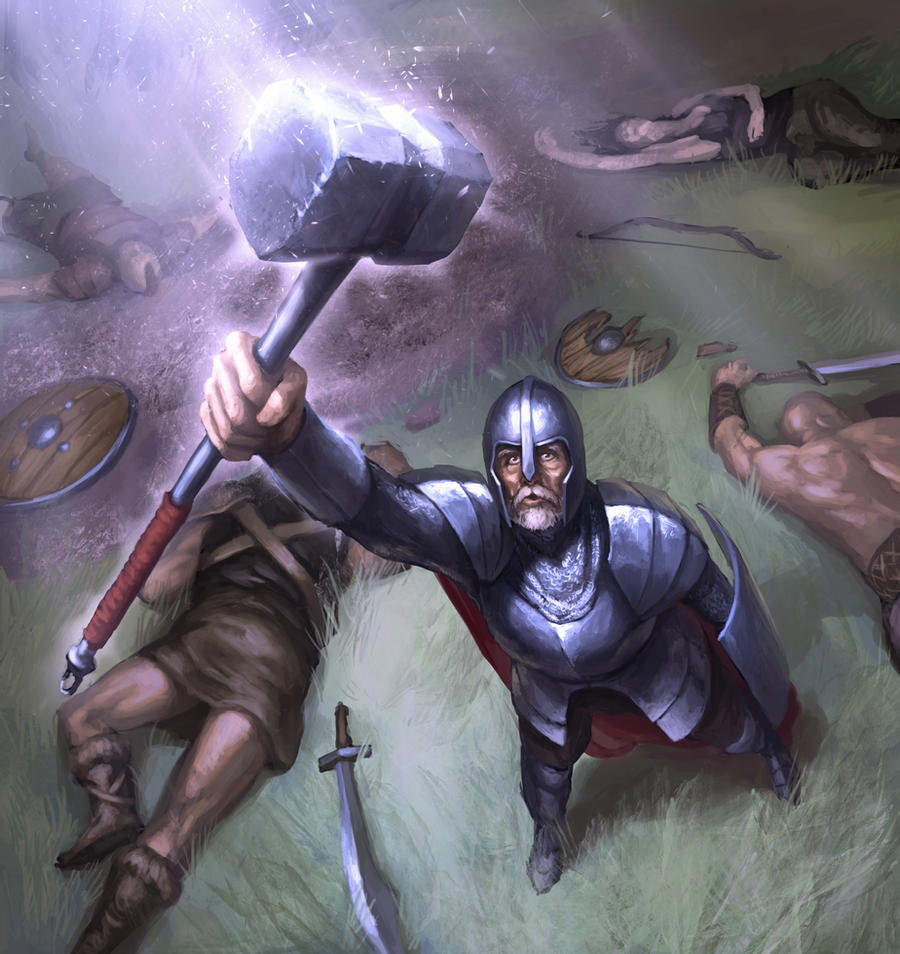
\includegraphics[scale=0.26]{img/invigorate_card_by_sirend.jpg}
\end{center}
\end{figure}



%\begin{samepage}
\begin{rpg-spell}
{Repair and Replace}
{Magnitude 2, Progressive, Instant\\{[Religions: Craft]}}

This spell repairs broken crafted items. It also replaces missing parts of an item. The size of the item depends on the Magnitude of the spell:
\begin{rpg-list}
\item 1 - Small items, such as pots, plates, knives, a defaced detail on a stone fresco, etc.
\item 2 - Medium. Large containers such as wine amphorae, target shields, longswords, human sized armour, a missing arm on a broken statue.
\item 3 - Large. Tower shields, broken doors, a missing masonry feature such as a column.
\item 4 - Huge. Giant armour, ruined houses, shattered towers.
\item 5 - Ginormous. The broken parts of a walking castle, the ruined walls of a city.
\end{rpg-list}
\end{rpg-spell}
%\end{samepage}

%\begin{samepage}
\begin{rpg-spell}
{Reflection}
{Duration 15, Magnitude 1, Progressive, Ranged\\{[Religions: Trickster]}}

This spell reflects incoming spells aimed at the target or his equipment, redirecting the spell back at the original caster. Once cast on a subject, Reflection will attempt to reflect any spells cast at the target. It will not have any effect on spells that are already affecting a character. The effects of Reflection depend on the relative Magnitude of both itself and the incoming spell. If the Reflection's Magnitude is equal or greater to the incoming spell then it is reflected and Reflection remains; if not Reflection is eliminated and the incoming spell takes effect. 

Reflection is incompatible with Absorption, Shield and Spirit Block.
\end{rpg-spell}
%\end{samepage}

%\begin{samepage}
\begin{rpg-spell}
{Resurrect}
{Concentration Special, Instant, Magnitude 5, Touch\\{[Religions: Death, Fertility, Sun]}}

The body of the deceased must be present and must be whole. If the target died due to disease or poison, the ailment must be eliminated or the Resurrect spell will fail. 

This spell summons the deceased spirit to return its former body. Resurrect takes a number of minutes equal to the target’s totalled Characteristics to take effect, during which time the caster must maintain concentration on the spell. If interrupted the spell fails. If the spell is completed without interruption the dead character returns to life with one hit point.

Resurrect must be cast within a number of days equal to the POW of the deceased. Casting the spell after this point results in the magic automatically failing. 
\end{rpg-spell}
%\end{samepage}

%\begin{samepage}
\begin{rpg-spell}
{Rout}
{Magnitude 3\\{[Religions: War]}}

When aimed at a body of warriors, no more than 100 persons, they make a Persistence roll or immediately lose all cohesion as a unit and rout. Routing units move at double movement, away from the caster to ideally a place of safety.  They will not defend themselves, but will attack any enemy units that get in their way, with the aim of getting through them to their place of safety.  
\end{rpg-spell}
%\end{samepage}

%\begin{samepage}
\begin{rpg-spell}
{See Past}
{Magnitude 2, Area, Concentration\\{[Religions: Knowledge]}}

When cast on a 10m area, the caster can see that area as it was in any past point of time he wishes. The can see for as long as they concentrate and they can not interact with the scene they see in any way, shape or form. They still need to make successful Perception rolls to notice details, such as important clues.
\end{rpg-spell}
%\end{samepage}

%\begin{samepage}
\begin{rpg-spell}
{Shield}
{Duration 15, Magnitude 1, Progressive\\{[Religions: War]}}

This spell protects the caster from physical and magical attacks. Each point of Magnitude gives the caster one Armour Point and provides a +10\% bonus to any tests the caster may make to resist malign magical effects. These effects are cumulative with other spells, as well as any physical armour the caster is wearing. Shield is incompatible with Absorption, Reflection and Spirit Block. 
\end{rpg-spell}
%\end{samepage}

%\begin{samepage}
\begin{rpg-spell}
{Soul Sight}
{Duration 15, Magnitude 1, Touch\\{[Religions: All]}}

This spell allows the recipient to see the POW aura of anyone he looks at, enabling them to discern that creature’s current Power Points, as well as the nature of any active spells or enchanted items the creature is carrying. It also allows the recipient to see into the Spirit World. 
\end{rpg-spell}
%\end{samepage}

%\begin{samepage}
\begin{rpg-spell}
{Spirit Block}
{Duration 15, Magnitude 1, Progressive, Touch\\{[Religions: All]}}

The recipient of Spirit Block may only be touched by Spirits with a POW high enough to break through the spell’s Magnitude; 1 - POW 10+, 2 - POW 17+, 3 - POW 26+, 4 - POW 37+, 5 - POW 50+, 6 - POW 65+, 7 - 82+, 8 - 101+.

A spirit unable to touch a Spirit Blocked character will not be able to personally attack or harm the recipient, including through ranged attacks (such as a thrown spectral javelin). A spell cast by a spirit at the recipient is blocked unless its Magnitude exceeds Spirit Block’s Magnitude. 

Spirit Block is incompatible with Absorption, Reflection and Shield. 
\end{rpg-spell}
%\end{samepage}

%\begin{samepage}
\begin{rpg-spell}
{Sun Disc}
{Magnitude 1, Ranged, Resist (Dodge)\\{[Religions: All]}}

Upon casting this spell, the caster projects a disc of blinding light (roll vs Dodge or be blinded for 1D4 hours) from their hand. Its warming effect melts ice upon contact, even magical ice if under three Magnitude in power, and gives anyone it touches +40\% resistance versus cold.
\end{rpg-spell}
%\end{samepage}

%\begin{samepage}
\begin{rpg-spell}
{Sunspear}
{Instant, Magnitude 4, Ranged, Resist (Dodge)\\{[Religions: Sun]}}

This spell will only function in direct sunlight. When cast, a shaft of light two metres wide streaks from the sky to blast a single target, who must be visible to the caster. If the target does not dive out of the way, the blazing light will burn it for 4D6 damage. Armour points are not effective against this damage and it counts as both magical and fire damage. 
\end{rpg-spell}
%\end{samepage}

%\begin{samepage}
\begin{rpg-spell}
{Summon Holy Steed}
{Magnitude 3, Duration 1 Day\\{[Religions: Various]}}

This spell summons a Holy Steed (see page~\pageref{monster:holy-steed}) from the Other World which is associated with the Deity that the Summoner worships. The Steed will obey the orders of the Summoner until the duration of the spell is up at which point the Steed will return to the Other World from whence it came. If the caster spends 3 Improvement Points when the Steed is summoned it remains in their service on a permanent basis, unless killed.
\end{rpg-spell}
%\end{samepage}

%\begin{samepage}
\begin{rpg-spell}
{Summon Holy Warrior}
{Magnitude 3, Duration 1 Day\\{[Religions: Various]}}

This spell summons a Holy Warrior (see page~\pageref{monster:holy-warrior}) from the Other World which is associated with the Deity that the Summoner worships. The Warrior will obey the orders of the Summoner until the duration of the spell is up at which point the Warrior will return to the Other World from whence it came. If the caster spends 3 Improvement Points when the Warrior summoned will remain in their service on a permanent basis, unless killed. Warriors are usually summoned to act as bodyguards, treasure guards and assassins.

Special powers for Warriors are available at the cost of increasing the spell’s Magnitude by 1. Typically these are random (roll 1D12):
\begin{rpg-list}
\item 1 - Additional mode of attack.
\item 2 - Extra set of arms, additional attack.
\item 3 - Extra natural weapon, eg. Horns D10 damage.
\item 4 - Breathes fire or ice or lighting (appropriate to elemental alliances of Deity) for D10 damage once per combat round.
\item 5 - Wings, therefore flies at 18 Move.
\item 6 - Hideous appearance that strikes fear into enemies (+40\% to Influence roll when Intimidating) or Beautiful appearance which charms all that behold them (+40\% to Influence rolls).
\item 7 - Mighty Divine weapons that does D20 damage.
\item 8 - Shapechanger.
\item 9 - Heavily armoured (9 AP instead of normal 6AP).
\item 10 - Can become insubstantial and walk through solid walls. While in this state can not interact with the real world.
\item 11 - Can become Invisible at will.
\item 12 - Faster, +18 Move, than normal.
\end{rpg-list}

Examples:

The Horned Horror of Yiko has Ranged Combat with a bow as an additional mode of attack, horns on its head which can be used as a weapon, and has a pair of wings, which means it requires a 6 Magnitude spell to summon it.

The Treasure Demon of Surlis-Sang, is a shapechanger that actually hides as the Treasure chest containing the treasure it is protecting, and so needs a 4 point spell to summon.
\end{rpg-spell}
%\end{samepage}

%\begin{samepage}
\begin{rpg-spell}
{Sureshot}
{Duration 15, Magnitude 1, Ranged\\{[Religions: Hunter]}}

Cast on a missile weapon (such as a knife, arrow, javelin or rock), this spell is triggered when it is fired. Unless the wielder of the weapon rolls an automatic failure or a fumble, the missile hits successfully (though it may be dodged or parried). So long as the target is within the maximum range of the weapon, the missile will strike home, regardless of concealment or any other factors. Attempts to parry or dodge the missile suffer a –20\% penalty. 

Sureshot may not be combined with Fire Missile, Multi Missile or Speedart – Sureshot will always take precedence in such cases. 
\end{rpg-spell}
%\end{samepage}

%\begin{samepage}
\begin{rpg-spell}
{Touch of Death}
{Magnitude 4, Touch, Instant, Resist (Persistence)\\{[Religions: Death]}}

The caster must touch their victim and on a failed Persistence test the victim falls down dead. This incredibly powerful spell is available to only members of religions whose Deity wield the power of Death itself. It is usually used to readdress the balance where a person who by all rights should be dead is still alive. 
\end{rpg-spell}
%\end{samepage}

%\begin{samepage}
\begin{rpg-spell}
{Treasury}
{Magnitude 4, Duration 1 Day\\{[Religions: Merchant]}}

This creates a secure room for one day, to store valuables in. All the entrances are locked and only the caster can come in and out without setting off a magical alarm that the caster can hear no matter how far away from the room.
\end{rpg-spell}
%\end{samepage}

%\begin{samepage}
\begin{rpg-spell}
{True (Weapon)}
{Magnitude 3, Duration 15, Ranged\\{[Religions: War]}}

Cast on the specified type of close combat weapon, this spell doubles that weapon’s normal damage dice. Other modifiers, such as Damage Modifier, are not affected. The wielder of the weapon should roll the weapon’s damage twice and total the result.
\end{rpg-spell}
%\end{samepage}

%\begin{samepage}
\begin{rpg-spell}
{Ward Camp}
{Magnitude 2, Duration 8 Hours, Area\\{[Religions: Merchant]}}

This spell protects a camp with an area of 10 square meters. Anyone crossing the invisible boundary of the spell takes 1D10 damage, and sets off a magical alarm that immediately awakens everyone within the camp.  The Ward stays in place, even after it has been crossed, for the full duration of the spell.
\end{rpg-spell}
%\end{samepage}

%\begin{samepage}
\begin{rpg-spell}
{War Effigy}
{Magnitude 4, Resist (Persistence)\\{[Religions: Trickster]}}

This spell enchants a small wax representation of the intended victim. Spells can be cast at the effigy and affect the victim, despite the distance between the effigy and the victim. The caster need not need have seen/met the victim,  since it is the power of their god that is providing the link. Once a day the victim can be caused physical harm by driving pins into the effigy, at 1D4 damage per pin. The caster can attempt to kill the victim outright by breaking off the head of the effigy. In this case the victim gets a Persistence roll to avoid death. On a failed Persistence test the victim dies. On a successful Persistence roll the effigy no longer has any power over the victim.
\end{rpg-spell}
%\end{samepage}

%\begin{samepage}
\begin{rpg-spell}
{Whirlwind}
{Magnitude 1, Progressive, Duration 15 Minutes\\{[Religions: Storm]}}

Each point of Magnitude of this spell whips up a whirlwind that is 10 metres tall and is capable of carrying 20 SIZ in its whirling vortex.  Each round the Whirlwind moves ten metres per point, in a random direction (use a D8 to determine direction, with 1 being North and 5 being South, progressing clockwise round the directions). 

If a character is hit by the Whirlwind, make a Dodge roll to avoid being caught up in it. Characters who are caught are whipped off their feet, D6 metres into the vortex. Each round roll a D6:
\begin{rpg-list}
\item 1-2: Carried up D10 metres (if already at the top, blown out the whirlwind the additional height before falliing to earth (taking damage).
\item 3-4: Stay at the height they are.
\item 5-6: Fall D6 down in the vortex. If this takes them to the ground they take falling damage.
\end{rpg-list}
\end{rpg-spell}
%\end{samepage}



